\begin{figure}[h]
    \centering
    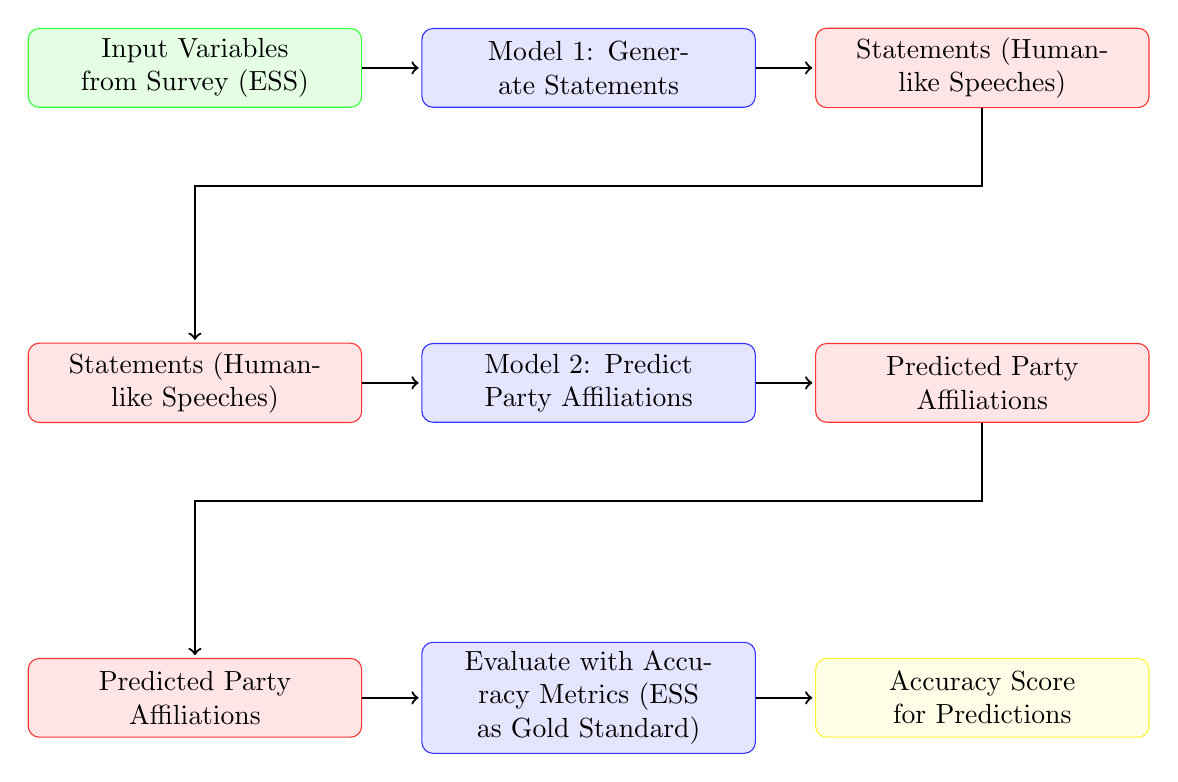
\begin{tikzpicture}[
      node distance=2.5cm and 2.5cm,
      every node/.style={fill=blue!10, rectangle, rounded corners, draw=blue!80, align=center, text width=4cm, minimum height=1cm},
      input/.style={fill=green!10, rectangle, rounded corners, draw=green!80},
      output/.style={fill=red!10, rectangle, rounded corners, draw=red!80},
      finaloutput/.style={fill=yellow!10, rectangle, rounded corners, draw=yellow!80},
      evaluation/.style={fill=blue!10, rectangle, rounded corners, draw=blue!80},
      every arrow/.style={draw, thick, ->, shorten >=1pt},
    ]

    % First row
    \node[input] (input1) {Input Variables from Survey (ESS)};
    \node (model1) [right of=input1, xshift=2.5cm] {Model 1: Generate Statements};
    \node[output] (output1) [right of=model1, xshift=2.5cm] {Statements (Human-like Speeches)};

    % Second row
    \node[output] (output1_dup) [below of=input1, yshift=-1.5cm] {Statements (Human-like Speeches)};
    \node (model2) [right of=output1_dup, xshift=2.5cm] {Model 2: Predict Party Affiliations};
    \node[output] (output2) [right of=model2, xshift=2.5cm] {Predicted Party Affiliations};

    % Third row
    \node[output] (output2_dup) [below of=output1_dup, yshift=-1.5cm] {Predicted Party Affiliations};
    \node[evaluation] (final_evaluation) [right of=output2_dup, xshift=2.5cm] {Evaluate with Accuracy Metrics (ESS as Gold Standard)};
    \node[finaloutput] (accuracy_score) [right of=final_evaluation, xshift=2.5cm] {Accuracy Score for Predictions};

    % Arrows
    \draw [every arrow] (input1) -- (model1);
    \draw [every arrow] (model1) -- (output1);
    \draw [every arrow] (output1) -- ++(0, -1.5) -| (output1_dup);
    \draw [every arrow] (output1_dup) -- (model2);
    \draw [every arrow] (model2) -- (output2);
    \draw [every arrow] (output2) -- ++(0, -1.5) -| (output2_dup);
    \draw [every arrow] (output2_dup) -- (final_evaluation);
    \draw [every arrow] (final_evaluation) -- (accuracy_score);

    \end{tikzpicture}
    \caption{The diagram illustrates the research methodology for survey imputation using Large Language Models (LLMs). Input variables from the ESS survey are transformed into human-like statements by Model 1. These statements are then used by Model 2 to predict party affiliations. The predicted affiliations are evaluated against the gold standard using accuracy metrics, with the final accuracy score for the predicted party affiliations being calculated.}
\end{figure}
